\input{preamble}
\input{format}
\input{commands}

\begin{document}

\begin{Large}
    \textsf{\textbf{Homework 3}}
    
    \textbf{Interpolation and Image Inpainting}
\end{Large}

\vspace{1ex}

\textsf{\textbf{Student:}} \text{Yuanyuan Zhao, 2300013077, School of EECS}, \href{mailto:your.email@hotmail.com}{\texttt{zhaoyuanyuan@stu.pku.edu.cn}}\\
\textsf{\textbf{Lecturer:}} \text{Yisong Chen}
% \href{mailto:your.email@hotmail.com}
% {\texttt{chenyisong@pku.edu.cn}}\\


\vspace{2ex}


\begin{problem}{Image Inpainting Program Design}{inpainting}
    Given 4  original-damaged image pairs, we need to designed a method to remove the Red Text on the damaged ones, in an effort to get closed to the original at most. Specific implementation can be found in the file: image\_inpainting.mlx.

\begin{enumerate}[(a)]
    \item \textbf{Build the Mask}
    \begin{enumerate}[label = (\roman*)]
        \item Based on our observation of the damaged images and their RGB values, the fact was found that all the damaging texts are pure red([255, 0, 0] in RGB). \\So we have
        \begin{verbatim}
        target_red = [255,0,0];
        \end{verbatim}
        

        \item Next, we need to find the damaged regions to be inpainted, to say, pixels whose RGB value == [255, 0, 0]. \\ So we have
        \begin{verbatim}
        mask = img_damaged(:,:,1)==target_red(1) &
        img_damaged(:,:,2)==target_red(2) &
        img_damaged(:,:,3)==target_red(3);
        \end{verbatim}
        This strict correspondence might be short of adaptiveness since in a real scenario what we are going to remove is not a pure color in all likelihood. In that case a threshold is needed and pixels within the target color range will get masked. But after all, the basic idea is to match those pixels with damaging features (e.g., pure red in this homework).
    \end{enumerate}

    
    \item \textbf{Inpaint the Masked Region}
        \begin{enumerate}[label = (\roman*)]
            \item After acquring the masked region, we call the function \texttt{regionfill(I, mask) } to replace masked pixel values using their neighbors. There are other inpainting methods such as \texttt{inpaintExemplar} in Matlab as well. But under comparison, \texttt{regionfill} seems to achieve the best performance despite some subtle inauthentic details which will be discussed later.
            \item Algorithm of \texttt{regionfill}: \texttt{regionfill} smoothly interpolates inward from the pixel values on the outer boundary of the regions. \texttt{regionfill} calculates the discrete Laplacian over the regions and solves the Dirichlet boundary value problem.\cite{regionfill_doc} Specific implementation details and principles will be discussed in the following section.
    \end{enumerate}
    
\end{enumerate}
\end{problem}

\begin{figure}[htbp]
    \centering 
    \begin{minipage}{0.8\textwidth} 
        \centering 
        
        \begin{subfigure}[b]{0.45\linewidth} 
            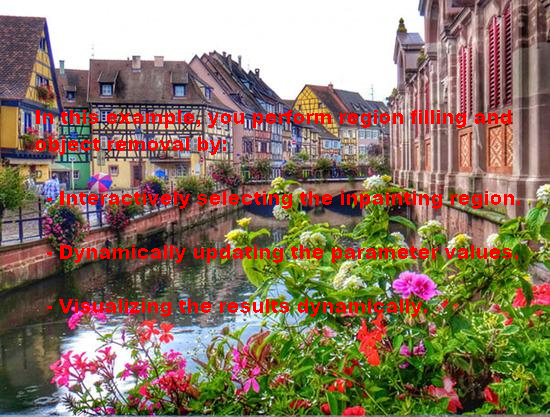
\includegraphics[width=\linewidth]{images/Colmar_damaged.png}
            \caption{Damaged Image}
        \end{subfigure}
        \hfill
        \begin{subfigure}[b]{0.45\linewidth}
            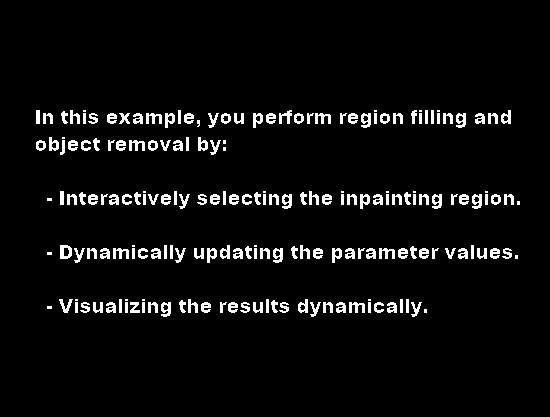
\includegraphics[width=\linewidth]{images/Colmar_mask.jpg}
            \caption{Mask}
        \end{subfigure}

        \vspace{0.5cm}
        \begin{subfigure}[b]{0.45\linewidth}
            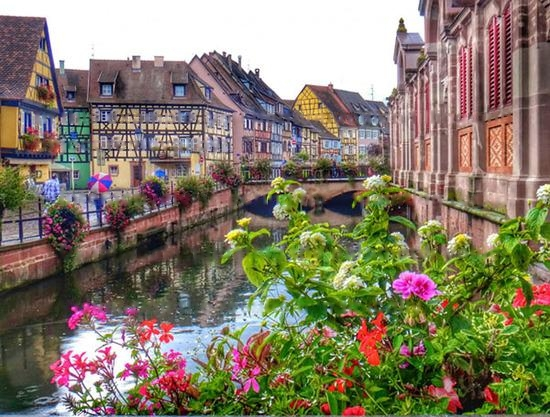
\includegraphics[width=\linewidth]{images/Colmar_inpainted.jpg}
            \caption{Inpainted Image}
        \end{subfigure}
        \hfill
        \begin{subfigure}[b]{0.45\linewidth}
            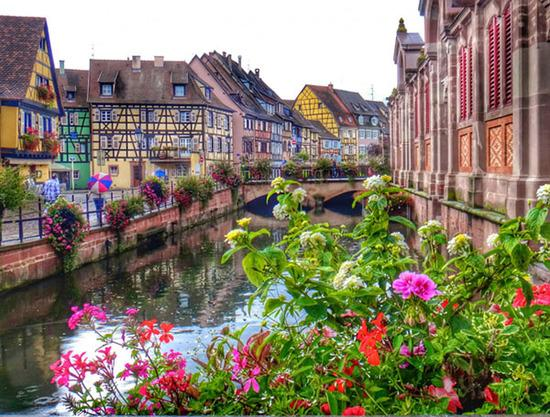
\includegraphics[width=\linewidth]{images/Colmar.jpg}
            \caption{Original Image}
        \end{subfigure}

        \caption{Colmar: Before, during and after inpainting}
        \label{fig:Colmar}
    \end{minipage}
\end{figure}

\begin{figure}[htbp]
    \centering 
    \begin{minipage}{0.8\textwidth} 
        \centering 
        
        \begin{subfigure}[b]{0.45\linewidth} 
            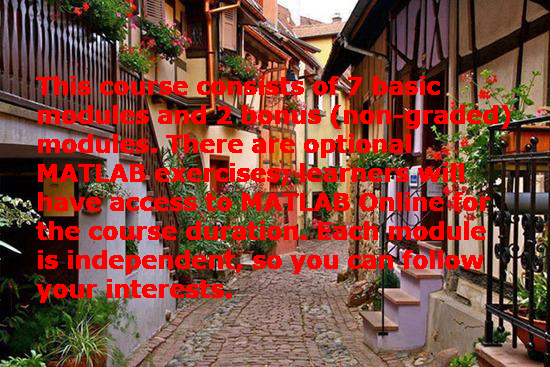
\includegraphics[width=\linewidth]{images/Eguisheim_damaged.png}
            \caption{Damaged Image}
        \end{subfigure}
        \hfill
        \begin{subfigure}[b]{0.45\linewidth}
            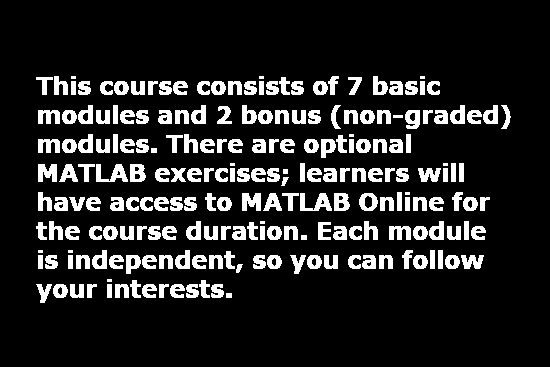
\includegraphics[width=\linewidth]{images/Eguisheim_mask.jpg}
            \caption{Mask}
        \end{subfigure}

        \vspace{0.5cm}
        \begin{subfigure}[b]{0.45\linewidth}
            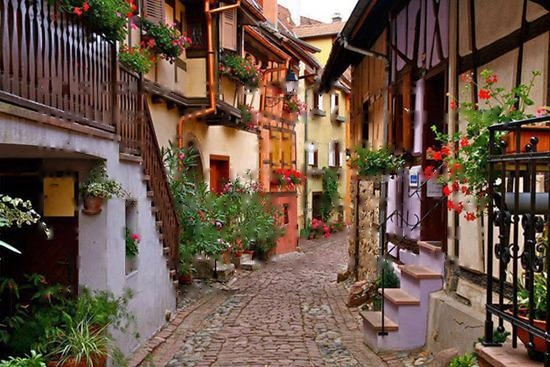
\includegraphics[width=\linewidth]{images/Eguisheim_inpainted.jpg}
            \caption{Inpainted Image}
        \end{subfigure}
        \hfill
        \begin{subfigure}[b]{0.45\linewidth}
            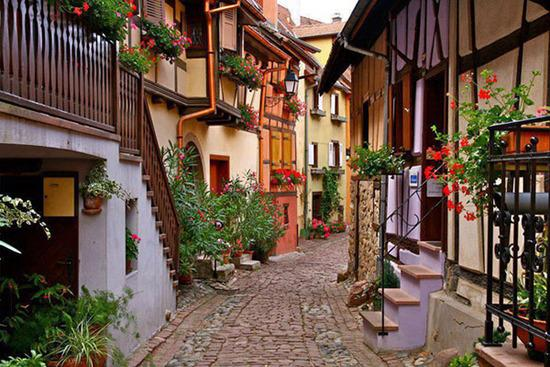
\includegraphics[width=\linewidth]{images/Eguisheim.jpg}
            \caption{Original Image}
        \end{subfigure}

        \caption{Eguisheim: Before, during and after inpainting}
        \label{fig:Eguisheim}
    \end{minipage}
\end{figure}

\begin{figure}[htbp]
    \centering 
    \begin{minipage}{0.8\textwidth} 
        \centering 
        
        \begin{subfigure}[b]{0.45\linewidth} 
            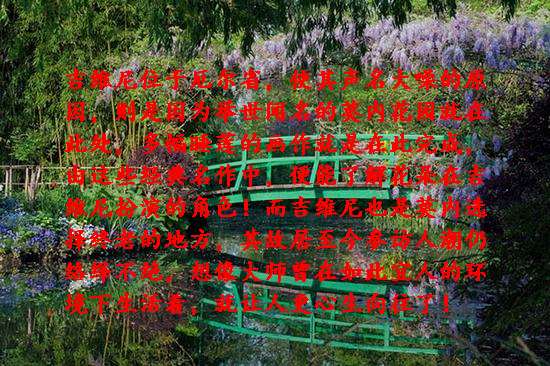
\includegraphics[width=\linewidth]{images/Giverny_damaged.png}
            \caption{Damaged Image}
        \end{subfigure}
        \hfill
        \begin{subfigure}[b]{0.45\linewidth}
            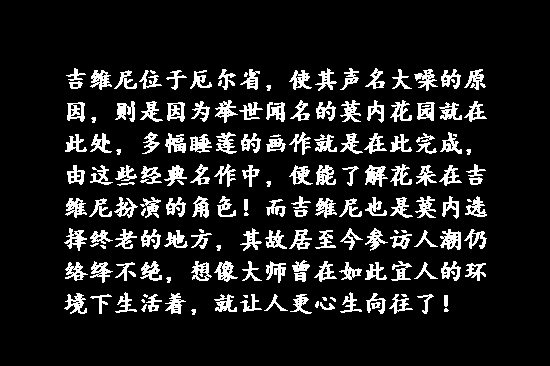
\includegraphics[width=\linewidth]{images/Giverny_mask.jpg}
            \caption{Mask}
        \end{subfigure}

        \vspace{0.5cm}
        \begin{subfigure}[b]{0.45\linewidth}
            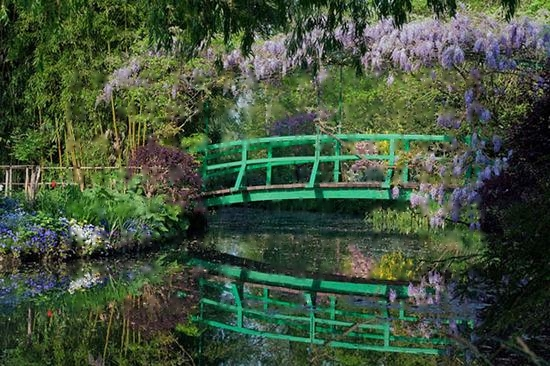
\includegraphics[width=\linewidth]{images/Giverny_inpainted.jpg}
            \caption{Inpainted Image}
        \end{subfigure}
        \hfill
        \begin{subfigure}[b]{0.45\linewidth}
            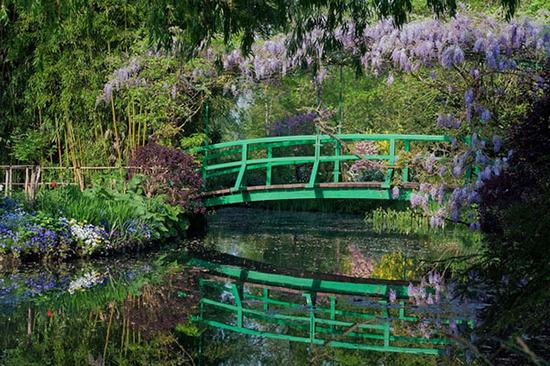
\includegraphics[width=\linewidth]{images/Giverny.jpg}
            \caption{Original Image}
        \end{subfigure}

        \caption{Giverny: Before, during and after inpainting}
        \label{fig:Giverny}
    \end{minipage}
\end{figure}

\begin{figure}[htbp]
    \centering 
    \begin{minipage}{0.8\textwidth} 
        \centering 
        
        \begin{subfigure}[b]{0.45\linewidth} 
            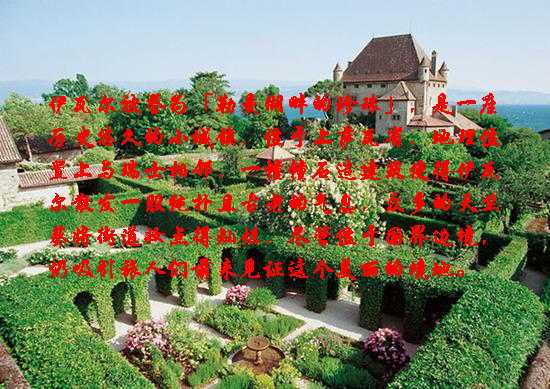
\includegraphics[width=\linewidth]{images/Yvoire_damaged.png}
            \caption{Damaged Image}
        \end{subfigure}
        \hfill
        \begin{subfigure}[b]{0.45\linewidth}
            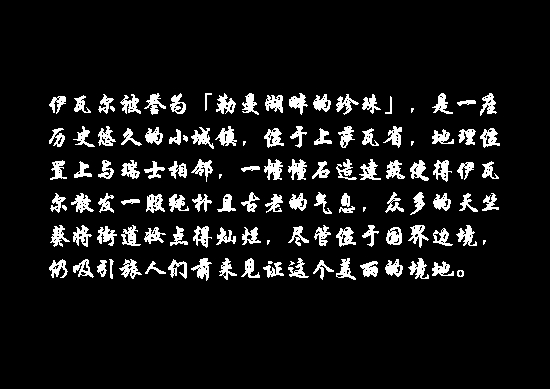
\includegraphics[width=\linewidth]{images/Yvoire_mask.jpg}
            \caption{Mask}
        \end{subfigure}

        \vspace{0.5cm}
        \begin{subfigure}[b]{0.45\linewidth}
            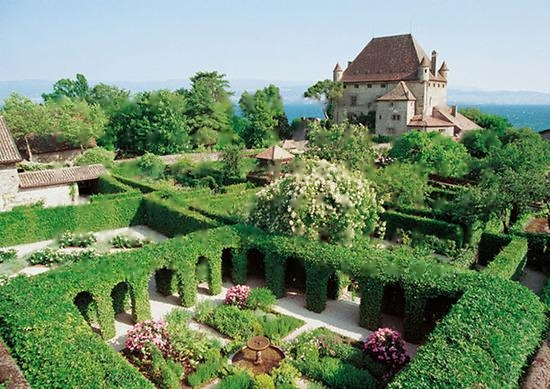
\includegraphics[width=\linewidth]{images/Yvoire_inpainted.jpg}
            \caption{Inpainted Image}
        \end{subfigure}
        \hfill
        \begin{subfigure}[b]{0.45\linewidth}
            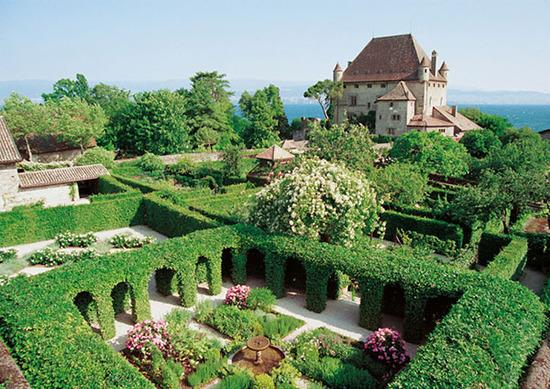
\includegraphics[width=\linewidth]{images/Yvoire.jpg}
            \caption{Original Image}
        \end{subfigure}

        \caption{Yvoire: Before, during and after inpainting}
        \label{fig:Yvoire}
    \end{minipage}
\end{figure}


\begin{problem}{Result Analysis}{result}

\begin{enumerate}[(a)]
    \item \textbf{Inpainted Images}\\ As shown in Figure \ref{fig:Colmar}, \ref{fig:Eguisheim}, \ref{fig:Giverny}, \ref{fig:Yvoire}, the ultimate results are satisfying at first glance. Yet when zooming in, we can still find them inauthentic somewhere. To be specific, traces of characters are still there despite the color integration with their surroundings. This is inevitably rooted in our inpainting algorithm, which will be elaborated on later.

    \item \textbf{Evaluations}\\As listed in Table \ref{table:evaluation}, the PSNR values are close to 30 dB, and the SSIM values are close to 1, both of which indicate that the inpainted images are highly similar to the original ones.
\end{enumerate}
\end{problem}

\begin{table}[]
    \centering
    \begin{tabular}{|l|l|l|l|l|}
        \hline
        Image Pairs & Colmar & Eguisheim & Giverny & Yvoire \\ \hline
        PSNR(dB)        & 32.51  & 27.44     & 29.31   & 29.5   \\ \hline
        SSIM        & 0.99   & 0.96      & 0.96    & 0.97   \\ \hline
    \end{tabular}
    \caption{PSNR and SSIM evaluation for each image pair}
    \label{table:evaluation}
\end{table}

\begin{problem}{Dive into \texttt{regionfill}}{regionfill}
\begin{enumerate}[(a)]
    \item \textbf{Implementation and Principles}\cite{Eddins2015}\\
        Image inpainting aims to reconstruct missing regions (e.g., scratches, occlusions) by propagating information from intact neighboring pixels. Laplace's equation naturally models this process.
        \begin{enumerate}[label = (\roman*)]
            \item Laplace's equation
                $$\frac{\partial^2 f}{\partial x^2} + \frac{\partial^2 f}{\partial y^2} = 0$$
                \textbf{Analogy to Steady-State Heat Flow}: Imagine heating the edges of a missing region; Laplace's equation ensures heat (or pixel intensity) diffuses evenly until equilibrium. This mimics how pixel values "diffuse" into gaps.\\
                \textbf{Smoothness Prior}: The equation enforces smooth transitions, avoiding sharp discontinuities. This is ideal for reconstructing textures or gradients (e.g., skies, skin tones).\\
                In a simple, discretized version of Laplace's equation, the value of every grid element in the interior of the region equals the average of its north, east, south, and west neighbors in the grid.
                $$\frac{\partial^2 f}{\partial x^2} = \frac{1}{h}[\frac{1}{h}(f(x+h,y)-f(x,y))-\frac{1}{h}(f(x,y)-f(x-h,y))]$$
                $$\text{let }h=1, \ \ \frac{\partial^2 f}{\partial x^2} + \frac{\partial^2 f}{\partial y^2} = 0$$
                $$\Rightarrow f(i,j) = \frac{1}{4}[f(i+1,j) + f(i-1,j) + f(i,j+1) + f(i,j-1)]$$
            \item Sparse Matrix Linear System\\
            Now we're going to set up a linear system of equations, $Ax=b$, so that the solution gives us every pixel of the output image. Let's think of the pixels as being numbered in columnwise order from 1 to the total number of pixels.
                \begin{verbatim}
                u = find(mask);
                v = ones(size(u));
                % for masked pixels, calculate the average
                ijv_mask = [...
                    u  u         1.00*v
                    u  u_north  -0.25*v
                    u  u_east   -0.25*v
                    u  u_south  -0.25*v
                    u  u_west   -0.25*v ];
                % for non-masked pixels, the original value
                ijv_nonmask = [w  w  1.00*ones(size(w))];
                ijv = [ijv_mask; ijv_nonmask];
                A = sparse(ijv(:,1),ijv(:,2),ijv(:,3));
                % b contains the original pixel values 
                % for pixels outside the mask
                % or 0 for pixels inside the mask
                b = I(:);
                b(mask(:)) = 0; 
                x = A\b;
                J2 = reshape(x,size(I)); % J2 is what we need
                \end{verbatim}
            
        \end{enumerate}
    \item \textbf{Strengths}
        \begin{enumerate}[label = (\roman*)]
            \item Computationally efficient.
            \item Preserves edges and gradients outside the masked region.
            \item Works well for small holes or smooth textures.
        \end{enumerate}
    \item \textbf{Limitations}
        \begin{enumerate}[label = (\roman*)]
            \item Struggles with large or complex missing regions (e.g., repetitive patterns).
            \item Fails to capture high-frequency details (e.g., fine textures).
            \item Assumes smoothness, which may oversimplify real-world images.
        \end{enumerate}

\end{enumerate}
\end{problem}

\begin{problem}{Thoughts}{thoughts}
    Interpolation is the underlying idea of a bunch of algorithms in digital image processing, and varying methods of interpolation design determine varying effects and corresponding applicable scenarios. For instance, Laplace's equation, as a kind of interpolation, achieves smoothness yet discard high-frequency details and that's the trade-off. \\
    Simple as interpolation may seem, it implies the widely-used idea of \textit{Knowing the unknown from what we've got}, paving the way for countless advanced algorithms we are familiar with, even the neural network.\\
    Exploring those behind a handy Matlab function call (e.g., \texttt{regionfill} in this report), I've discovered something beyond the Matlab documents, to say, the blogs recording the whole procedure of a function implementation. And that's exactly where I got some invaluable insights.
\end{problem}


% =================================================

% \newpage

% \vfill

\bibliographystyle{ieeetr}
\bibliography{references}

\end{document}